\section{Results}
\label{subsec:cupid-results}
% A number of examples of the application of \ac{CUPID} are now presented.
% Each result was obtained using the same procedure. For every region of interest
% in the dataset, a frequency-filtered \ac{FID} was produced. An initial estimate
% of model order was determined either using the \ac{MDL}, or by hard-coding a
% value determined through manual inspection of the \ac{2DJ} spectrum\footnote{
%     The \ac{MDL} was used in circumstances where it provided reasonable
%     predictions of model order, as less user input needs to be given to the
%     routine when this is so. However, in certain situations when the \ac{MDL}
%     performed inadequately\,---\,most commonly when the
%     region being considered was very crowded\,---\,a manual specification
%     needed to be provided.
% }.
% An estimation result was then generated using the \ac{MMEMPM} followed by
% phase-variance regularised \ac{NLP}. Finally, a suitable frequency threshold
% $\epsilon$ was determined, and any oscillators in the parameter estimate which
% abided by the two criteria in \cref{subsec:mp-selection} were removed.

A number of examples of the application of \ac{CUPID} are now presented.
For details relating to generation of the presented datasets, see
\cref{sec:simulated-datasets,subsec:cupid-experimental,subsec:psyche-datasets}.
Useful metrics, such as run times and the number of oscillators present at
different stages of the estimation routine are provided in
\cref{tab:cupid-metrics}.

\subsection{``Four Multiplets''}
\label{subsec:four-mp}
\begin{figure}
    \centering
    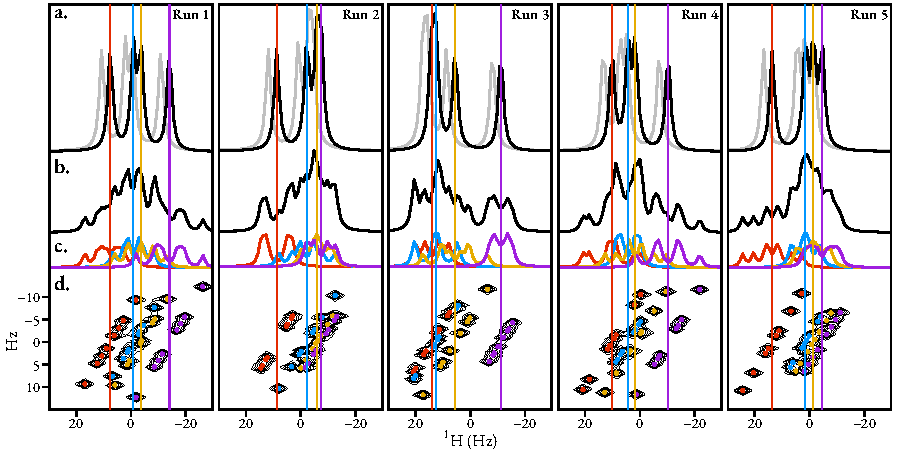
\includegraphics{four_multiplets/four_multiplets}
    \caption[
        The result of applying \acs{CUPID} on 5 instances of simulated
        \acs{2DJ} datasets with 4 heavily overlapping multiplet structures.
    ]{
        The result of applying \ac{CUPID} on 5 instances of simulated \ac{2DJ}
        datasets with 4 heavily overlapping multiplet structures.
        \textbf{a.} Black: pure shift spectrum generated by \ac{CUPID} (via the
        \ang{-45} signal).
        Grey: \ac{1D} spectrum simulated with \textsc{Spinach}, using the same spin
        system as was used to produce the \ac{2DJ} dataset, but with all scalar
        couplings set to \qty{0}{\hertz}. This has been offset slightly for
        clarity.
        \textbf{b.} \ac{1D} spectrum of the dataset, produced using the first
        direct-dimension \ac{FID} in the \ac{2DJ} dataset.
        \textbf{c.} Multiplet structures predicted, using the threshold $\epsilon
        = \nicefrac{\fswtwo}{\Ntwo} \approx \qty{0.98}{\hertz}$.
        \textbf{d.} Contour plot of the \ac{2DJ} spectrum in magnitude-mode,
        with coloured points denoting the frequencies of oscillators in the
        estimation result. The coloured vertical lines denote the predicted
        central frequencies of each multiplet structure.
    }
    \label{fig:four-multiplets}
    \vspace{20pt}
    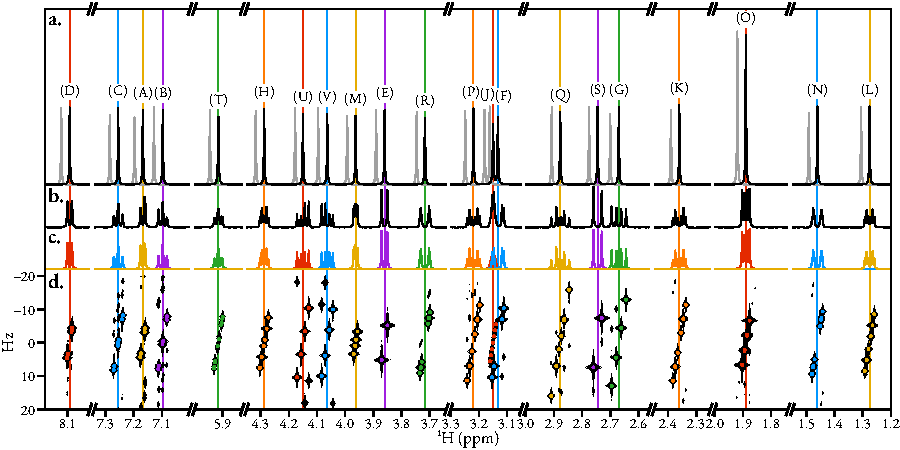
\includegraphics{strychnine_cupid/strychnine_cupid.pdf}
    \caption[
        The application of \acs{CUPID} on a simulated strychnine \acs{2DJ}
        dataset.
    ]
    {
        The application of \ac{CUPID} on a simulated strychnine \ac{2DJ} dataset.
        See \cref{fig:four-multiplets} for a description of the panels.
        The multiplet structures were assigned using the threshold
        $\epsilon = \nicefrac{\fswtwo}{\Ntwo} \approx \qty{0.39}{\hertz}$.
    }
    \label{fig:strychnine-cupid}
\end{figure}

A series of five simulated \ac{2DJ} datasets
were generated using \textsc{Spinach} such that within a
known region of the spectrum, four ddd multiplet
structures with significant overlap were present. \ac{AWGN} was added to each
\ac{FID}, with a target \ac{SNR} of \qty{30}{\deci\bel}.
Filtering was applied to the datasets to generate sub-\acp{FID} containing the
signals in the region of interest
(\SIrange{-30}{30}{\hertz}).
\cref{fig:four-multiplets} provides an illustration of \ac{CUPID}'s performance
when applied to the datasets.
Each of the sub-\acp{FID} comprised 32 ($4 \times 2^3$) signals.
As can be seen in \cref{fig:four-multiplets}.b, the first direct-dimension
\acp{FID} are too crowded for reasonable estimates of model
order to be made using the \ac{MDL}, so a value was manually provided; for each
dataset, a random
integer from the range $[33, 40]$ was selected as the initial number of
oscillators. Hence, the initial guess from the \ac{MMEMPM} comprised a
slightly excessive number of oscillators in each case.
For each \ac{FID} generated, \ac{CUPID} was able to produce a
result with 32 oscillators, as desired, despite the excessive number
that were present in the initial guess. Most of the excessive oscillators were
purged during the \ac{NLP} procedure through their acquisition of negative
amplitudes.
For 2 of the 5 datasets, the result after \ac{NLP} comprised 33
oscillators, with a single oscillator being associated with noise remaining.
These were be automatically detected and removed using the first-order signal
detection criteria described in \cref{subsec:mp-selection}.

With simulated examples such as this, it is possible to confirm that the pure
shift spectrum generated using \ac{CUPID} agrees with the expected result; the
``true'' pure shift spectrum can be obtained by simulating a pulse-acquire
experiment, using a spin system with same chemical shifts, but with all J-couplings
set to \qty{0}{\hertz}. As seen in \cref{fig:four-multiplets}.a. the spectra
produced using \ac{CUPID} agree well with these. Beyond pure shift spectrum
generation, the multiplet assignment was also successful; each of the ddd
structures were resolved, and these are plotted in
\cref{fig:four-multiplets}.c.

% \subsection{Sucrose simulated}
% \label{subsec:sucrose-cupid}
% \note{Maybe not so impressive? Perhaps try strychnine?}
% \begin{figure}
%     \centering
%     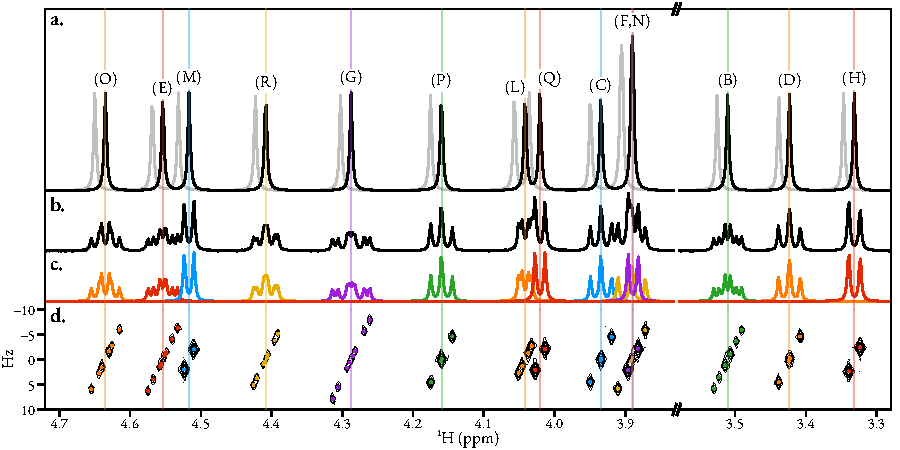
\includegraphics{sucrose_cupid/sucrose_cupid.pdf}
%     \caption[
%         The application of \acs{CUPID} on a simulated sucrose \acs{2DJ} dataset.
%     ]
%     {
%         The application of \ac{CUPID} on a simulated sucrose \ac{2DJ} dataset.
%         \textbf{a.} Black: the spectrum generated from \ac{FT} of the \ang{-45}
%         signal. Grey: the spectrum of a simulated dataset with the same
%         chemical shifts, with all scalar couplings set to \qty{0}{\hertz}.
%         \textbf{b.} Conventional \ac{1D} spectrum.
%         \textbf{c.} Multiplet structures assigned ($\epsilon \approx
%         \qty{0.27}{\hertz}$).
%         \textbf{d.} Contour plot of the absolute value mode \ac{2DJ} spectrum,
%         with the locations of assigned oscillators given as coloured points.
%     }
%     \label{fig:sucrose-cupid}
% \end{figure}
% As a second example of applying \ac{CUPID} on simulated data, the chemical
% shifts and isotropic scalar couplings associated with a
% Gaussian\cite{Gaussian03} \ac{DFT} calculation of sucrose in a vacuum
% \footnote{
% It is well known that isotropic chemical shift calculations using \ac{DFT} are
% typically very inaccurate. The resulting spectrum is not typical of sucrose in
% the liquid state, though this doesn't really matter for assessing the
% performance of \ac{CUPID}.
% }
% were used to construct a 2DJ dataset. \ac{AWGN} was added with a target
% \ac{SNR} of \qty{20}{\deci\bel}. The CUPID procedure was applied to filtered
% sub-FIDs such that the signals arising from all 22 spins were considered, though
% only the regions of the dataset with the most interesting multiplet structures
% are presented in \cref{fig:sucrose-cupid}.

% The estimation technique successfully assigned multiplet structures for all 22
% multiplets in the dataset, including structures derived from two spins (F \& N)
% with a \qty{0.6}{\hertz} difference in resonance frequency, approaching the
% spectral resolution in the direct dimension (\qty{0.537}{\hertz}). The
% pure-shift spectrum generated via the \ang{-45} signal again showed close
% agreement with a 1D spectrum simulated using the same chemical shifts, with
% scalar couplings set to \qty{0}{\hertz}. There are particular multiplets where
% the number of oscillators fit using the estimation routine was less than the
% true number. Examples of this phenomenon are exhibited in the estimates of the
% multiplets for spins B \& O, which are both ddd structures. The scalar
% couplings involved meant that certain oscillators were
% of such similar frequencies that they were separated by significantly less than
% the spectral resolution, and thus resolving these was unrealistic. For
% example, there are two pairs of peaks in the spin-B multiplet which lie only
% \qty{0.085}{\hertz} apart. Under-fitting in this case had a negligible impact
% on the final pure shift spectrum. However there are circumstances which will be
% seen in the experimental examples below where more blatant cases of under-fitting
% lead to the generation of peaks in the pure shift spectrum which are noticeably
% broadened.

\subsection{Strychnine Simulated}
\label{subsec:strychnine-cupid}
As a second example of applying \ac{CUPID} on simulated data, the chemical
shifts and isotropic scalar couplings associated with strychnine
were used to construct a 2DJ dataset. \ac{AWGN} was included with a target
\ac{SNR} of \qty{20}{\deci\bel}. CUPID was applied to filtered
sub-FIDs such that the signals arising from all spins were considered, with the
result presented in \cref{fig:strychnine-cupid}. There are numerous
regions in the dataset where strong coupling artefacts reside, and as such this
dataset provides a good gauge on the effectiveness of \ac{CUPID} when these are
present.

The \ac{MDL} was applied to the first direct-dimension \acp{FID} in order to
predict their model orders. In most circumstances, the model order used resulted
in estimation results in which the first-order signals were well
quantified, while those corresponding to strong coupling artefacts were neglected.
In some circumstances, certain strong couplings signals were quantified, though
the relevant oscillators were purged on every occasion based on the first-order
criteria. As such, no such artefacts appear in the final pure shift spectrum.
The absence of strong coupling artefacts in the estimation result also leads to
generated multiplet structures which do not exhibit the typical ``roofing''
effect associated with strongly coupled spins (\textit{cf.} Figures
\ref{fig:strychnine-cupid}.b and \ref{fig:strychnine-cupid}.c). The clearest
examples of this are associated with the pair (U) and (V), as well as the trio (A),
(B) and (C). As with the four multiplets example, good agreement is achieved
between the pure shift spectrum generated via the \ang{-45} signal, and a
spectrum generated by running a \ac{1D} simulation with the same spin system,
expect that scalar couplings are set to \qty{0}{\hertz}.

\subsection{Quinine}
\begin{figure}
    \centering
    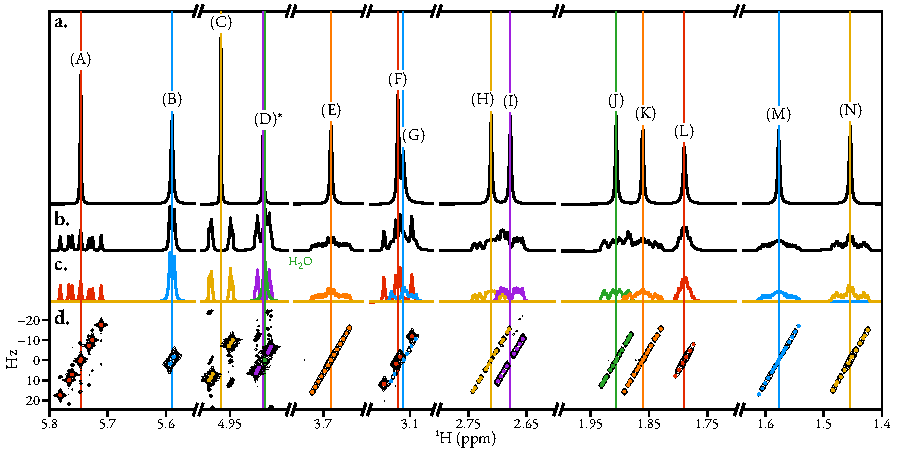
\includegraphics{quinine_cupid/quinine_cupid.pdf}
    \caption[
        The application of \acs{CUPID} on a quinine \acs{2DJ} dataset.
    ]{
        The application of \ac{CUPID} on the non-aromatic regions of a quinine
        \ac{2DJ} dataset.
        \textbf{a.} Structure of quinine.
        \textbf{b.} Spectrum produced using the \ang{45} shear and projection
        approach. The peaks denoted by an asterisk originate from strong
        coupling artefacts.
        \textbf{c.} The spectrum generated from \ac{FT} of the \ang{-45}
        signal, with the signal arising from H\textsubscript{2}O (grey, close
        to \qty{4.9}{\partspermillion}) neglected.
        \textbf{d.} Spectrum of the first direct-dimension signal in the
        \ac{2DJ} \ac{FID}.
        \textbf{e.} Multiplet structures assigned ($\epsilon =
        \nicefrac{\fswtwo}{\Ntwo} \approx \qty{0.92}{\hertz}$).
        \textbf{f.} Contour plot of the \ac{2DJ} spectrum in magnitude-mode,
        with the locations of assigned oscillators given as coloured points.
    }
    \label{fig:quinine-cupid}
\end{figure}

\Cref{fig:quinine-cupid} illustrates the result of applying \ac{CUPID} on
a dataset generated from a sample comprising quinine (\cref{fig:structures}.f)
in \ch{CD3OD},
with all signals arising from non-aromatic protons considered.

For comparison with \ac{CUPID}, \cref{fig:quinine-cupid}.a shows the
spectrum produced using the shear-and-project method. Because
sine-bell apodisation was applied to the \ac{FID} in order to suppress dispersive
contributions, the relative amplitudes of the pure-shift
peaks are drastically different. In particular, the signals from the alkenyl
spins (A), (C) and (D) are attenuated less by apodisation relative to the
aliphatic signals due to their longer $T_2$ times\footnote{
    Spins with longer $T_2$s produce signals which decay less rapidly.
    Sine-bell apodisation heavily diminishes the intensities of the initial
    points in the \ac{FID}. Therefore, if the signal decays less rapidly, the
    relative extent by which the power of the signal is diminished is less
    compared with a signal derived from a spin with a small $T_2$.
}. As well as this, signals arising from strong coupling between (C) and
(D) are visible (these are denoted with an asterisk).

\ac{CUPID} successfully generated a pure shift spectrum with distinct peaks for
each \ch{^1H} environment, which possess sharper lines and more consistent
integrals relative to the shear-and-project spectrum (\cref{fig:quinine-cupid}.b).
Furthermore, the strong coupling artefacts between (C) and (D) were not
incorporated into the estimation result, and as such a clean baseline between
between (C) and (D) was achieved.
The multiplet grouping procedure was able to resolve
the signals corresponding to spin (D) (purple) from the singlet corresponding
to residual water in the sample (grey).
To obtain a clean signal for spin (D), without heavy overlap with the water
signal, the oscillator corresponding to the water was simply neglected from
the parameter set used to generate the \ang{-45} signal. This concept of
neglecting nuisance signals through post-processing has similarities with
\ac{SVD}-based approaches for solvent suppression\cite{Zhu1997}.
These methods operate by assuming that the most significant component(s) in the
data are derived from the solvent; these are subtracted from the dataset to
remove their influence. The process of removing the water signal from the quinine
data is slightly different, since it was suppressed manually through
inspection of the \ac{CUPID} result. A knowledgeable user would be able to
locate the water signal and discard it. However, in scenarios where little is
known about the sample, or the user does not have a high level of expertise,
manually neglecting signals in this manner may not be achievable.

This example provides a few examples where a noticeable under-fitting of
certain multiplet structures has occurred.
The most notable case comes from the spin (G) multiplet, where close proximity
with spin (F)'s multiplet has likely compounded the task of accurately
estimating the associated signals. With fewer oscillators than the true number
of signals at its disposal, the \ac{NLP} routine has compensated
by giving said oscillators large amplitudes and damping factors, so that they
can reasonably fit multiple similar-frequency signals. In these situations,
pure shift peaks generated via the \ang{-45} signal will possess augmented
linewidths.
This behaviour is also exhibited to a lesser extent by the multiplet for spin
(B), which comprises two pairs of very close signals in a dd structure. A
single oscillator is fit to each of the doublets, culminating in a slightly
broadened pure shift peak.


\subsection{Camphor}

\begin{figure}
    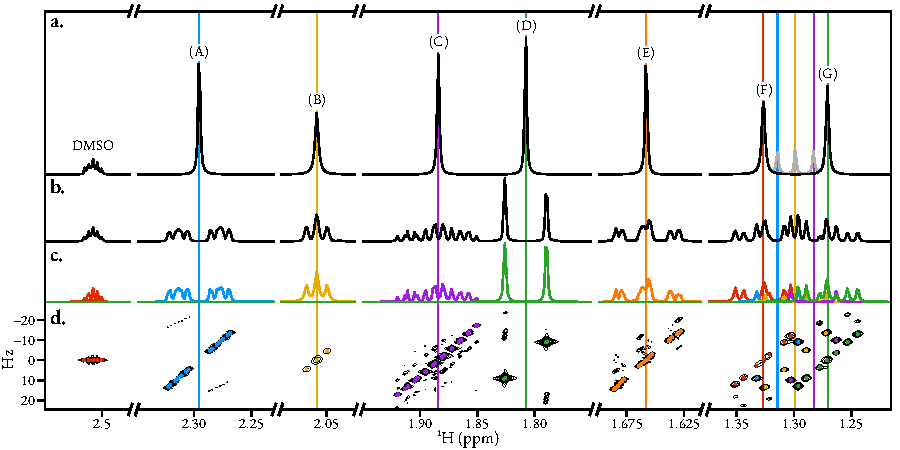
\includegraphics{camphor_cupid/camphor_cupid.pdf}%
    \caption[
    The application of \acs{CUPID} on a camphor \acs{2DJ} dataset.
    ]{
        The application of \acs{CUPID} on a camphor \ac{2DJ} dataset.
        \textbf{a.} Structure of camphor.
        \textbf{b.} Spectrum produced using the \ang{45} shear and projection
        approach. The peaks denoted by an asterisk originate from strong
        coupling artefacts.
        \textbf{c.} Black: spectrum generated from \ac{FT} of the \ang{-45}
        signal, by neglecting the strong coupling artefacts associated with
        spins (F) and (G).
        Grey: equivalent spectrum, but with the strong coupling artefacts
        incorporated.
        \textbf{d.} Spectrum of the first direct-dimension signal in the
        \ac{2DJ} \ac{FID}.
        \textbf{e.} Multiplet structures assigned ($\epsilon =
        \nicefrac{2\fswtwo}{\Ntwo} \approx \qty{1.23}{\hertz}$).
        \textbf{f.} Contour plot of the \ac{2DJ} spectrum in magnitude-mode,
        with the locations of assigned oscillators given as coloured points.
    }
    \label{fig:camphor-cupid}%
\end{figure}

The application of \ac{CUPID} to the non-methyl signals of a \ac{2DJ}
dataset of camphor (\cref{fig:structures}.f) in \acs{DMSOd6} is presented
in \cref{fig:camphor-cupid}. As with the quinine example, a spectrum
generated through the shear-and-project approach is presented for
comparison. In most regions of the dataset, the estimation technique
successfully parametrised the first-order signals, while neglecting strong
coupling artefacts. However, it was not possible to solely estimate the
first-order signals associated with the pair of spins (F) and (G). The extent
of strong coupling between the nuclei is such that some of the strong coupling
artefacts have comparable amplitudes to the first-order signals. Reliance on
the
\ac{MMEMPM}, which determines the most significant components in
the data, therefore makes it challenging to solely estimate the first-order
signals in this case. The strong coupling signals which were estimated by the
routine are denoted in grey in the \SIrange{1.36}{1.24}{\partspermillion} region
of the spectrum. Their contributions to the spectrum of the \ang{-45} signal
are also plotted in grey. As with the shear and summation spectrum, three extra
peaks reside between the pure shift peaks associated with (F) and (G), which
ideally would not exist. In much the same way that the parameters associated
with water in the quinine example were neglected in constructing the \ang{-45}
signal, those associated with strong coupling artefacts can be too.
In neglecting said parameters, the black spectrum in \cref{fig:camphor-cupid}.b
results. Again, achieving this requires manual intervention, with the user
requiring knowledge about the sample to distinguish between first-order signals
and strong coupling artefacts.

\subsection{Dexamethasone}
\begin{sidewaysfigure}%
    \centering%
    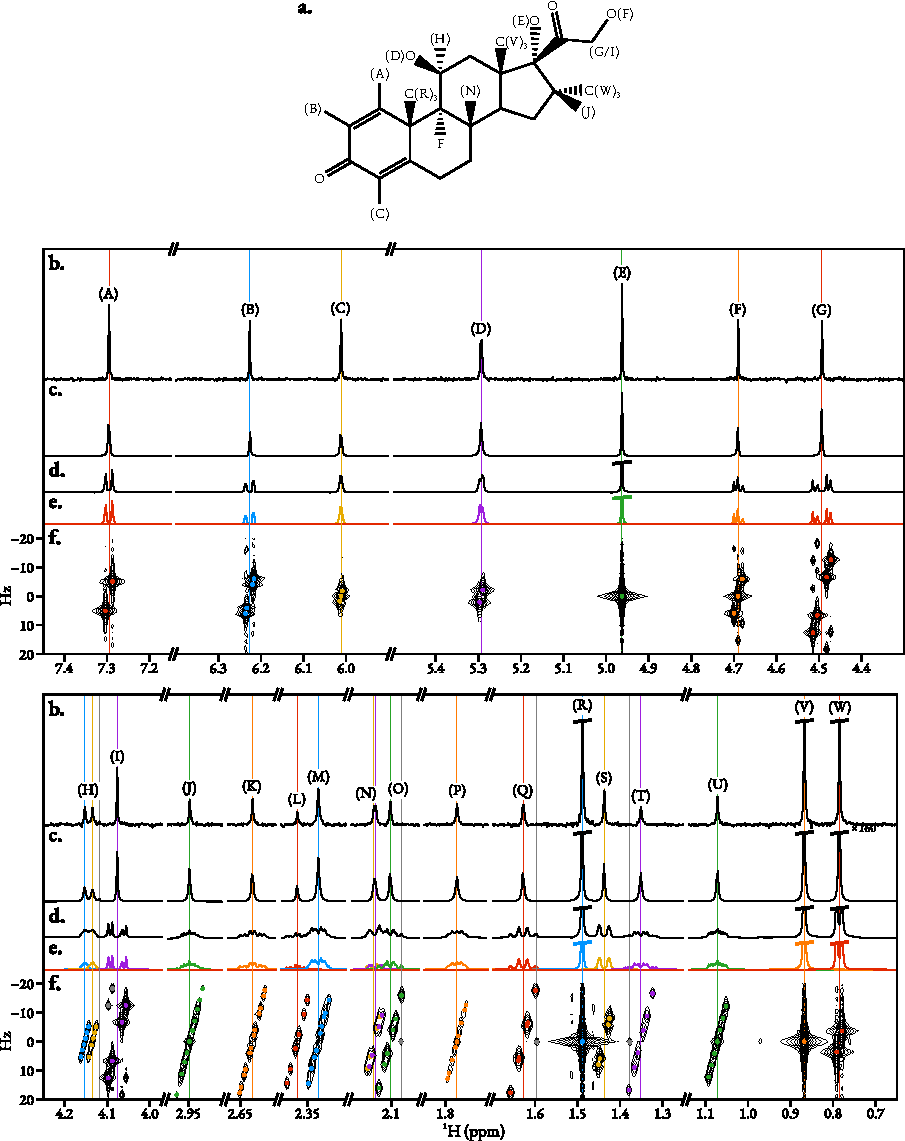
\includegraphics{dexamethasone_cupid/dexamethasone_cupid.pdf}%
    \caption[
        The application of \acs{CUPID} on a dexamethasone \acs{2DJ} dataset.
    ]{
        The application of \acs{CUPID} on a \ac{2DJ} dataset of dexamethasone in
        \acs{DMSOd6}.
        \textbf{a.} \acs{TSE-PSYCHE} spectrum.
        \textbf{b.} The spectrum generated from \ac{FT} of the \ang{-45}
        signal.
        \textbf{c.} Conventional \acs{1D} spectrum.
        \textbf{d.} Multiplet structures assigned ($\epsilon =
        \nicefrac{\fswtwo}{\Ntwo} \approx \qty{0.92}{\hertz}$).
        \textbf{e.} Magnitude-mode \acs{2DJ} spectrum, with the locations of
        assigned oscillators given as coloured points.
    }
    \label{fig:dexamethasone-cupid}%
\end{sidewaysfigure}%

\Cref{fig:dexamethasone-cupid} shows the result of applying CUPID on a
dataset acquired from a sample of dexamethasone (\cref{fig:structures}.h) in
DMSO-d\textsubscript{6}. A
pure shift spectrum was also acquired using the
\ac{TSE-PSYCHE} experiment\cite{Foroozandeh2018,Foroozandeh2015} for
comparison.
Overall, excellent agreement is achieved between the \ac{PSYCHE}
spectrum, and that generated using the \ang{-45} signal. The estimation routine
performed amicably even in cases where heteronuclear coupling to
\ch{^{19}F} exists. For spins (H) and (N), two distinct
multiplet structures were assigned, which are coloured blue and yellow (H), and
yellow and purple (N) in the figure. However, the very small though perceptible
heteronuclear coupling between \textsuperscript{19}F and (D) could not be
resolved.

In this example, there are a few cases where oscillators which correspond to
strong coupling artefacts exist in the final parameter set, even after applying
the first-order signal criteria. These persist because either they have an
indirect frequency
$\approx \qty{0}{\hertz}$ (these exist close to
\qty{1.4}{\partspermillion}, \qty{1.6}{\partspermillion}, and
\qty{2.1}{\partspermillion}), or because at
least two parameterised artefacts are grouped together as part of the multiplet
assignment (this occurs close to \qty{4.1}{\partspermillion}). As with the
camphor example, a knowledgeable user could identify and neglect the culprit
oscillators if desired, though they are not purged in producing the \ang{-45}
signal in this case to illustrate their effect on the final pure shift spectrum.

\subsection{Estradiol}
\begin{figure}
    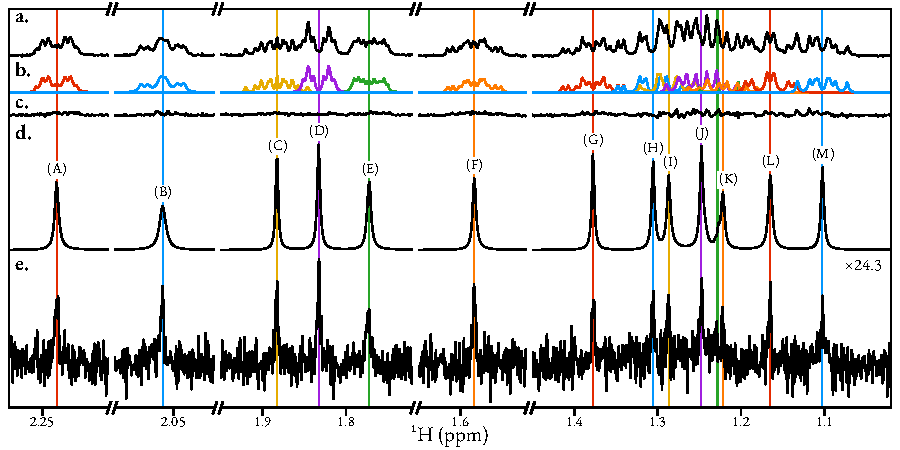
\includegraphics{estradiol_cupid/estradiol_cupid.pdf}%
    \caption[
        The application of \acs{CUPID} on a 17\textbeta-estradiol \acs{2DJ}
        dataset.
    ]{
        The application of \acs{CUPID} on a \ac{2DJ} dataset of 17\textbeta-estradiol
        in \acs{DMSOd6}.
        \textbf{a.} Structure of estradiol.
        \textbf{b.} \acs{PSYCHE} spectrum.
        The spectrum has been scaled such that its maximum is of the same
        magnitude as the \acs{CUPID} spectrum.
        \textbf{c.} Pure shift spectrum generated via the \ang{-45} signal.
        \textbf{d.} Conventional \ac{1D} spectrum.
        \textbf{e.} Multiplet structures assigned ($\epsilon =
        \qty{2}{\hertz}$).
        \textbf{f.} Magnitude-mode \ac{2DJ} spectrum, with coloured points
        denoting the frequencies of oscillators assigned using estimation.
        N.B. This \ac{2DJ} spectrum was produced using a more
        concentrated sample of estradiol, since the \ac{2DJ} dataset which
        \ac{CUPID} was applied on was too insensitive to produce a viable
        spectrum after sine-bell apodisation.
    }
    \label{fig:estradiol-cupid}%
\end{figure}

A final illustration of \ac{CUPID}'s performance is provided by
\cref{fig:estradiol-cupid} (\cref{fig:structures}.i),
where a low concentration (\qty{2}{\milli\molar}) sample of
17\textbeta-estradiol (\cref{fig:structures}.d) in \acs{DMSOd6} is
considered. This is the most challenging example presented due
to (a) the low \ac{SNR} of the data, and (b) the presence of incredibly complex
regions for a small molecule spectrum, featuring many overlapping
multiplet structures. In fact, because of the considerable complexity
of the estradiol \ac{1D} spectrum, the molecule was used to showcase the
\ac{PSYCHE} experiment in the original work describing
it\cite{Foroozandeh2014}.

The \ac{PSYCHE} experiment produced a spectrum with very poor
\ac{SNR}, such that it is barely sensitive enough for pure shift peaks to be
distinguished from the noise. However due to the innately higher
sensitivity associated with the \ac{2DJ} experiment it was still possible to
generate a reasonable parameter estimate of the \ac{2DJ} dataset, and
subsequently to yield an agreeable pure shift spectrum via the \ang{-45}
signal. Due to the severe signal overlap in the first
direct-dimension \ac{FID}, model order estimates had to be
manually specified. It is clear from inspection of the most downfield region
that certain strong coupling artefacts have been incorporated into the
estimation result, manifesting in the appearance of artefacts in the pure shift
spectrum (see the positions marked by the grey vertical lines in
\cref{fig:estradiol-cupid}.b).
The time elapsed to run the estimation routine was rather
long, at \qty{10.25}{\minute} for all regions considered (see
\cref{tab:cupid-metrics} for a more detailed run-down of timings). This is
largely attributable to the high model orders required in estimating the
spectral regions considered, particularly for the most downfield region (this
region alone took over \qty{5.5}{\minute} to estimate).
